\subsection{Radiacón Solar}

\subsubsection{El Sol}

\subsubsection{La Constante Solar}

\subsubsection{Distribución Espectral de Radiación Extraterrestre}

\subsubsection{Variación de Radiación Extraterrestre}
Cuando se estudian las variaciones de radiación extraterrestre, es necesario tomar en consideración la energía emitida por el sol. Se han identificado diferentes periodicidades y variaciones de intensidad, asociadas con la actividad de manchas solares. \\

También es necesario tomar en cuenta el impacto que tiene la órbita elíptica de la tierra con respecto al sol, la distancia entre estos dos varía causando una variación en el flujo de radiación solar en el rango del $\pm3.3\%$ \\

Existen dos modelos frecuentemente usados para calcular esta variación, el primero es razonablemente bueno para aplicaciones poco rigurosas o cotidianas, este modelo es descrito a través de la siguiente ecuación,

\begin{equation}
		G_{on} = G_{sc}\left(1 + 0.033 \cos \frac{360n}{365}\right) 
\end{equation}

Si se necesita más precisión, la siguiente expresión ofrece un $\pm0.01\%$ de variación,

\begin{align}
	\begin{aligned} \label{eq:variacion_extraterrestre_precisa}
		G_{on} & = G_{sc} \left(1.000110 + 0.034221 \cos B + 0.001280 \sin B \right.	\\
		& \left. + 0.000719 \cos 2B + 0.000077 \sin 2B \right)
	\end{aligned}
\end{align}

en dónde $G_{on}$ es la radiación incidente en el plano normal a la radiación dado un día $n$ del año. $B$ está dado por,

\begin{equation}
	B = \left(n - 1\right) \frac{360}{365}
\end{equation}

Usando la ecuación \ref{eq:variacion_extraterrestre_precisa}, obtenemos la siguiente gráfica.

\begin{figure}[htbp]
	\centering
	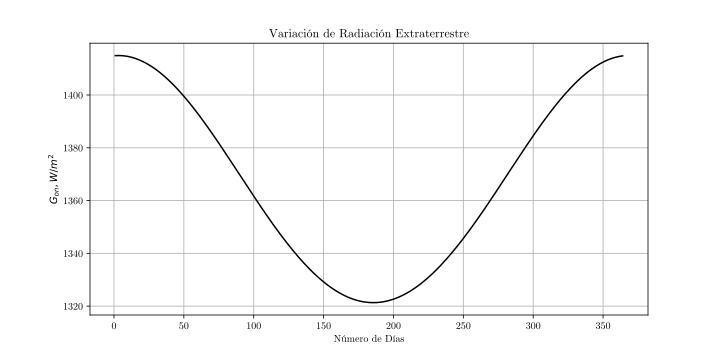
\includegraphics[width=0.8\textwidth, angle=0]{images/variationextraterrestrialsolarradiation.pdf}
	\caption{Variación de radiación solar extraterrestre en el plazo de un año.}
\end{figure}

\subsubsection{Dirección del Haz de Radiación}

Las relaciones geométricas de cualquier plano con respecto a cualquier orientación relativa a la tierra, en cualquier momento y un haz entrante de radiación solar, pueden ser descritas por varios ángulos, estos por convención son nombrados y se hace referencia hacia ellos como se muestra a continuación,

\begin{itemize}
	\item $\phi$ \textbf{Latitud}, es la ubicación angular al norte o sur del ecuador, siendo la dirección del norte positiva; $-90^\circ\leq\phi\leq90^\circ$.
	\item $\delta$ \textbf{Declinación}, es la posición angular del sol al medio día solar con respecto al plano del ecuador, por ejemplo, cuando este se encuentra en la meridiana local. Esta es positiva al norte; $-23.45^\circ\leq\delta\leq23.45^\circ$.
	\item $\beta$ \textbf{Pendiente}, es el ángulo entre el plano de la superficie en cuestión y la superficie; $0^\circ\leq\beta\leq180^\circ$.
	\item $\gamma$ \textbf{Ángulo de Acimut de Superficie}, es la desviación de la proyección en un plano horizontal a la superficie desde la meridiana local. $-180.0^\circ\leq\gamma\leq180.0^\circ$.
	\item $\omega$ \textbf{Ángulo de Hora}, el desplazamiento angular del sol del este o el oeste con respecto a la meridiana local debido a la rotación de la tierra cuyo valor es de $15^\circ$ por hora; En la mañana es negativo y en el atardecer positivo.
	\item $\theta$ \textbf{Ángulo de Incidencia}, es el ángulo entre el haz de radiación en una superficie y la normal de esa superficie.
	\item $\theta_z$ \textbf{Ángulo Cenital}, es el ángulo entre la vertical y la línea hacia el sol, en otras palabras, es el ángulo de incidencia del haz de radiación en una superficie horizontal.
	\item $\alpha_s$ \textbf{Ángulo de Altitud Solar}, es el ángulo entre la horizontal y la línea hacia el sol, es el complemento del ángulo cenital.
	\item $\gamma_s$ \textbf{Ángulo de Acimut Solar}, es el desplazamiento angular del sur de la proyección del haz de radiación en un plano horizontal. Los desplazamientos del este al sur son negativos y del oeste al sur son positivos.	
\end{itemize}

\begin{figure}[htbp]
	\centering
	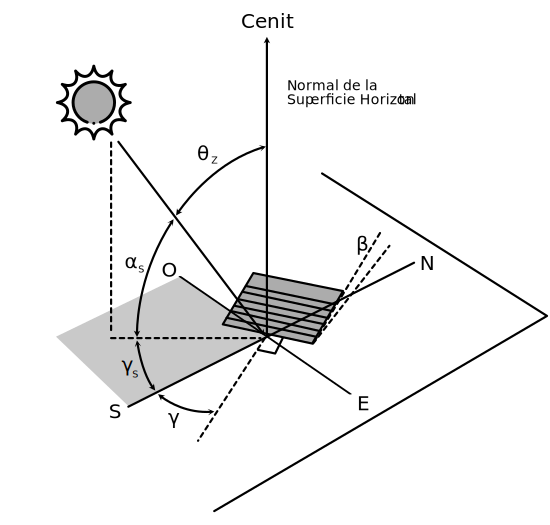
\includegraphics[width=0.6\textwidth, angle=0]{images/solarradiationdirectionangles.pdf}
	\caption{Ángulos de radiación solar.}
\end{figure}

\paragraph{La Declinación $\delta$}
Este ángulo puede ser encontrado a través de una aproximación como la que se muestra a continuación,
\begin{equation} \label{eq:declinacion_ingenieria}
\delta = 23.45 \sin\left( \frac{360}{365}\left( 284 + n\right) \right) 
\end{equation}
Para fines de ingeniería, la aproximación anterior resulta suficiente, sin embargo disponemos de otro modelo cuya precisión es mayor ya que el error es menor al $0.035^\circ$.

\begin{align} \label{eq:declinacion_precisa}
	\begin{aligned}
		\delta & = 0.006918 - 0.399912\cos\left(\Gamma \right) + 0.070257\sin(\Gamma) \\
		& -0.006758\cos\left(2\Gamma \right)  + 0.000907\sin\left(2\Gamma \right)  \\
		& -0.002697\cos\left(3\Gamma \right) + 0.00148\sin\left(3\Gamma \right)
	\end{aligned}
\end{align}

en dónde,
\begin{equation}
\Gamma = \frac{2\pi\left(n-1 \right) }{365}
\end{equation}

En ambas expresiones la variable $n$ es el número del día del año que se estudia, esta satisface $1\leq n \leq 365$.

\begin{figure}[htbp]
	\centering
	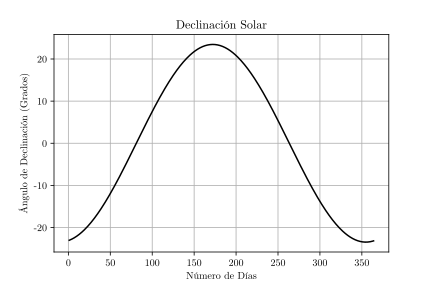
\includegraphics[width=0.8\textwidth, angle=0]{images/solardeclination.pdf}
	\caption{Diagrama de declinación solar.}
\end{figure}

Observando la interacción y dependencias entre ángulos, podemos deducir las siguientes relaciones que podemos utilizar para efectuar nuestros cálculos de posición.

\begin{align}
	\begin{aligned}
		\cos\theta & = \sin \delta \sin \phi \cos \beta - \sin \delta \cos \phi \cos \gamma \\
		& + \cos \delta \cos \phi \cos \beta \cos \omega + \cos \delta \sin \phi \sin \beta \cos \gamma \cos \omega \\
		& + \cos \delta \sin \beta \sin \gamma \sin \omega
	\end{aligned}
\end{align}
Y la siguiente expresión,
\begin{align}
	\begin{aligned}
		\cos\theta & = \cos \theta_z \cos \beta + \sin \theta_z \sin \beta \cos\left(\gamma_s - \gamma \right) 
	\end{aligned}
\end{align}

El ángulo $\theta$ puede exceder $90^\circ$, lo cuál significa que el sol se encuentra detrás de la superficie. \\

Con las relaciones expuestas anteriormente, se puede entonces tener un rastreo preciso de la posición del sol con respecto a un punto en la tierra usando la latitud y el día del año en el que se decide hacer la evaluación.